\section{Peripheral Recover and SCCP}	\label{sec:periRec}
%%\vspace{-5pt}
%

















To impletement REMARK, NVP is enhanced by four hardware modules to support flexible B/R functions and realize efficient peripheral recovery.

%\vspace{5pt}
\noindent\textbf{Backup/Restore (B/R) Manager.} \\
Existing NVP only supports passive B/R functions, which limits the flexibility of NVP.
Passive backup operation can only be triggered when the supply voltage is below the threshold.
When power recovers, passive restore operation is activated automatically and no initiator program is allowed. 
Target on these challenges, B/R Manager extends active B/R functions to support flexible checkpointing.
Moreover, a Bootstrap module is also added to support the initiator program.
The structure of the B/R Manager is shown in Fig.~\ref{fig:HardwareArchitecture}.

%
The B/R controller is enhanced by control logics which are used to select the trigger signal of B/R functions.
Two instructions, \emph{ABR} and \emph{EBR} (Table~\ref{tab:InstrSet}), are added to enable the active B/R functions.
Active backup is realized by \emph{ABR 1}, and active restore is \emph{ABR 0}.
In addition, \emph{EBR 0} and \emph{EBR 1} are used to disable and enable the B/R function, respectively.

%
Bootstrap is a module used to control the system clock and the reset signals.
Its work flow is shown in Fig.~\ref{fig:InitiatorFlow}.
After the system is powered on, Bootstrap selects whether to enter the restart procedure or to start the program from the very beginning according to the \emph{$1^{st}\_start$} signal.
\emph{$1^{st}\_start$} is an external signal set by users.
If \emph{$1^{st}\_start$} is set, the processor is started from the very beginning.
Otherwise, Initiator is started to recover the peripherals and restore the processor.
%Bootstrap generates the system clock for the processor and resets the modules before the entire system starts.
%Bootstrap can also gate the system clock when an active backup function is invoked.

%
\begin{figure}[t]
    \centering
    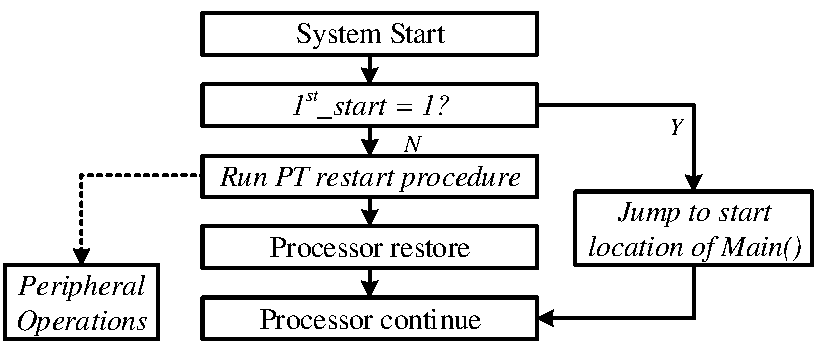
\includegraphics[width=0.48\textwidth]{Fig9_InitiatorFlow.pdf}
    %\vspace{-10pt}
    \caption{The flow chart of Initiator.}
    \label{fig:InitiatorFlow}
\end{figure}

%\vspace{5pt}
\noindent\textbf{Interrupt Recognizer (IRec).} \\
%
Interrupt is an interaction between processor and the peripherals where careful checkpoints should be placed.
IRec provides hardware support for reliable interrupt recovery.
It recognizes the interrupt request and decides whether to recover the interrupt.
Fig.~\ref{fig:HardwareArchitecture} shows the hardware diagram of this module.
Firstly, IRec contains a nonvolatile special register to store a programmable control bit, IR, which indicates whether an interrupt is recoverable.
If the interrupt is recoverable, IR is set and the system will recover the interrupt as a normal processor task.
Otherwise, IR is reset.
When an unrecoverable interrupt request arrives, the control logic triggers B/R Manager to execute a backup operation and set a checkpoint before the interrupt.
In this way, the system will resume from the checkpoint and skip the interrupt after power failure.

%\vspace{5pt}
\noindent\textbf{Peripheral Status Registers {(PSRs)}.} \\
PSRs are used to monitor the peripheral status in real-time to support efficient peripheral reconfiguration.
PSRs in Fig.~\ref{fig:HardwareArchitecture} is a group registers, each bit of which indicates whether a peripheral is ready or not.
These states will be set when the peripherals are configured and cleared after power failures.
Thus, a group of volatile registers are the ideal choice.
Since the internal registers are all non-volatile and are resumed after power failures, PSRs are added as external registers.
%When the system recovers after power failures, PSRs will be reset by the reset signal generated by the B/R Manager.

PSRs can be accessed by the processor with the proposed instruction \emph{RSR} and \emph{WSR} as shown in Table~\ref{tab:InstrSet}.
\emph{RSR} reads the value from \emph{SRaddr} into the register \emph{oper2}.
\emph{SRaddr} is the address of PSRs and has an independent address space from the register file.
\emph{oper2} can be the address of a normal register, a direct address or an indirect address.
Similarly, \emph{WSR} writes the value of second operand \emph{oper1} into \emph{SRaddr}.
\emph{oper1} can be the address of a normal register, a direct address, an indirect address or an immediate operand.

%\vspace{5pt}
\noindent\textbf{Peripheral Restart Module (PRM).} \\
PRM is used to locate the start function of peripherals and realize correct returning during the restarting procedure.
As shown in Fig.~\ref{fig:HardwareArchitecture}, PRM contains a special register \emph{EndAddr}, an XOR gate and the control logic.
When a peripheral needs to be restarted, PRM is called by the processor with two instructions.
Firstly, the end address of the peripheral start function is stored to \emph{EndAddr}.
Then, the program jumps to the peripheral start function with a \emph{JAL} instruction.
When the program counter reaches the end address, the XOR gate generates a positive trigger and the control logic enables a \emph{JR \$ra} instruction automatically.
In this way, the peripheral is successfully restarted and the program returns correctly to restart the next peripheral.